\section{Experiment Design}	\label{sec:experiments}
	In this paper, author have consider five different senarios to see how well the communication is between two callers (peers). 
	
	In the senario 1 (\hyperref[fig:scene-1]{Figure \ref{fig:scene-1}}), peer `A' (IP::10.127.204.227) and peer `B' (IP::10.127.10.203) are calling from same lab/office. Which let them connect at the same access point. Now, since both callers are at the same location we expect jitter to be very minimal and same send/receive loss at the both peers. In the \hyperref[fig:scene-out-1]{Figure \ref{fig:scene-out-1}} we can see the sending jitter at both peers have very same pattents. However there jitter vaules heigher then other. And this could happen due to the device that are been used are different. 
	\begin{figure}[thb]
		\begin{minipage}{\textwidth}
%			\vspace{2mm}
			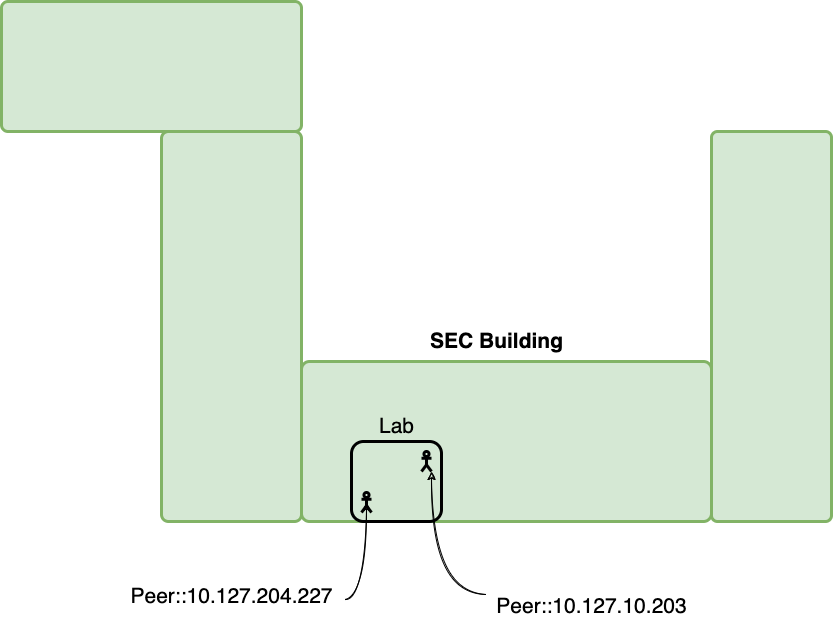
\includegraphics[scale=0.29]{Images/experiment/senarios/in_lab.drawio.png}
%			\vspace{2mm}
		\end{minipage}
		\caption{Senario 1: Two peers within same office}
		\label{fig:scene-1}
	\end{figure}

	\begin{figure}[!t]
		\begin{minipage}{\textwidth}
			%			\vspace{2mm}
			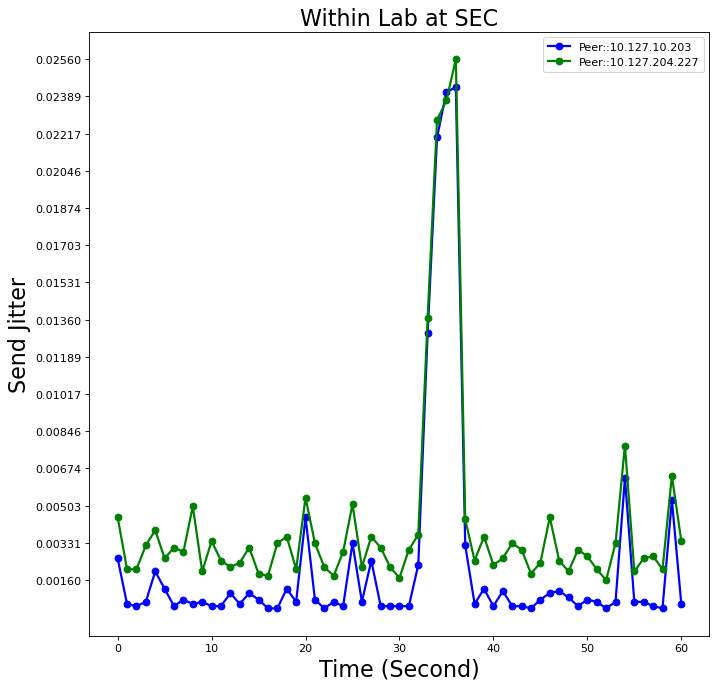
\includegraphics[scale=0.38]{Images/experiment/senarios/df_in_lab.png}
			%			\vspace{2mm}
		\end{minipage}
		\caption{Jitter values for the time spend by callers}
		\label{fig:scene-out-1}
	\end{figure}


	In the senario 2 (\hyperref[fig:scene-2]{Figure \ref{fig:scene-2}}), peer `A' (IP::10.127.204.227) and peer `B' (IP::10.127.10.203) are calling from different loaction. Peer `A' is staying at same lab/office and peer `B' is continuly moving into different locations with the same floor as peer `A'. This can let peer `B' change it's access point within same local area network. 
	\begin{figure}[thb]
		\begin{minipage}{\textwidth}
			%			\vspace{2mm}
			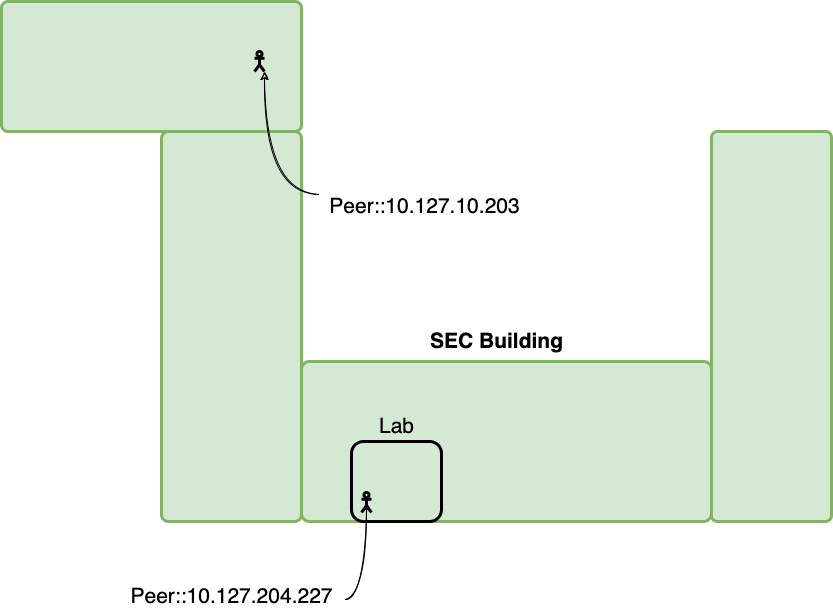
\includegraphics[scale=0.29]{Images/experiment/senarios/in_floor.drawio.png}
			%			\vspace{2mm}
		\end{minipage}
		\caption{Senario 2: Two peers within same floor}
		\label{fig:scene-2}
	\end{figure}

	\begin{figure}[!t]
		\begin{minipage}{\textwidth}
			%			\vspace{2mm}
			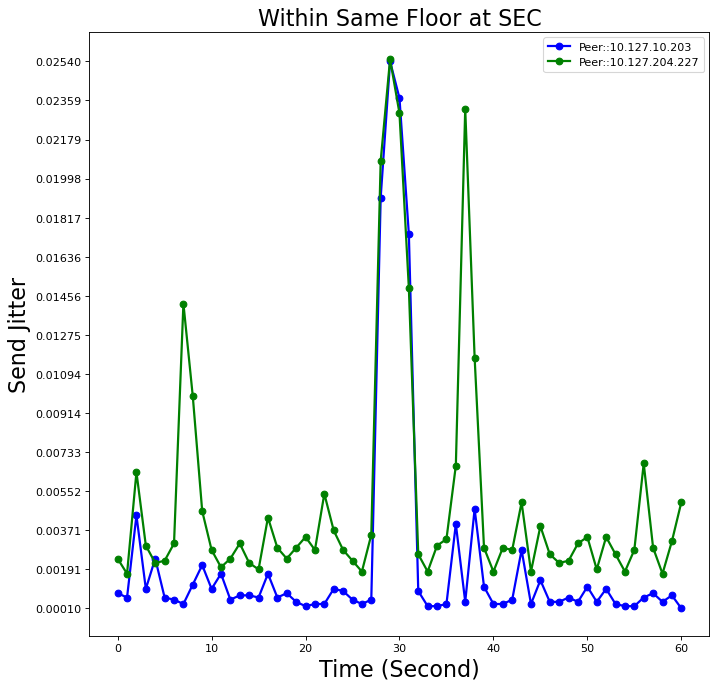
\includegraphics[scale=0.38]{Images/experiment/senarios/df_in_floor.png}
			%			\vspace{2mm}
		\end{minipage}
		\caption{Jitter values for the time spend by callers}
		\label{fig:scene-out-2}
	\end{figure}

	In the senario 3 (\hyperref[fig:scene-3]{Figure \ref{fig:scene-3}}), peer `A' (IP::10.127.204.227) and peer `B' (IP::10.127.10.203) are calling from different loaction.
	\begin{figure}[hb]
		\begin{minipage}{\textwidth}
			%			\vspace{2mm}
			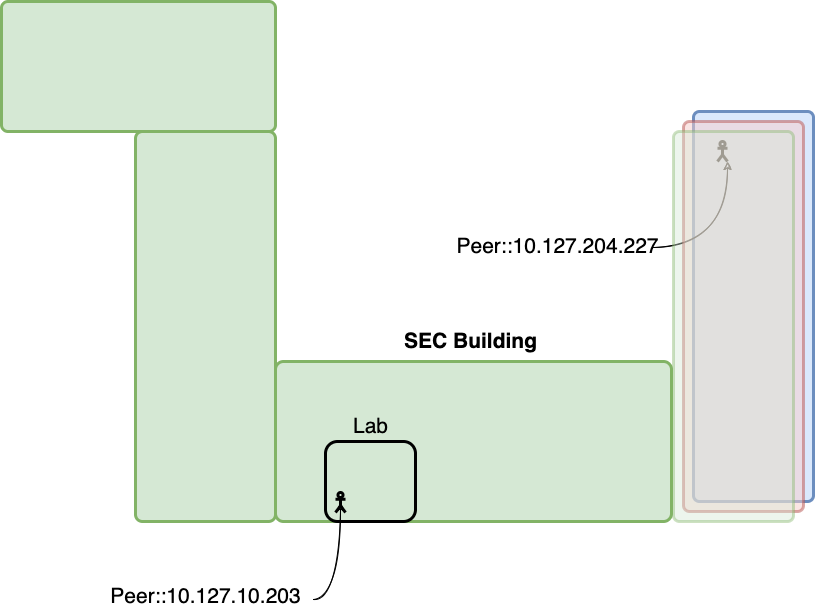
\includegraphics[scale=0.29]{Images/experiment/senarios/diff_floor.drawio.png}
			%			\vspace{2mm}
		\end{minipage}
		\caption{Senario 3: Two peers at different floors but within building}
		\label{fig:scene-3}
	\end{figure}

	\begin{figure}[!t]
		\begin{minipage}{\textwidth}
			%			\vspace{2mm}
			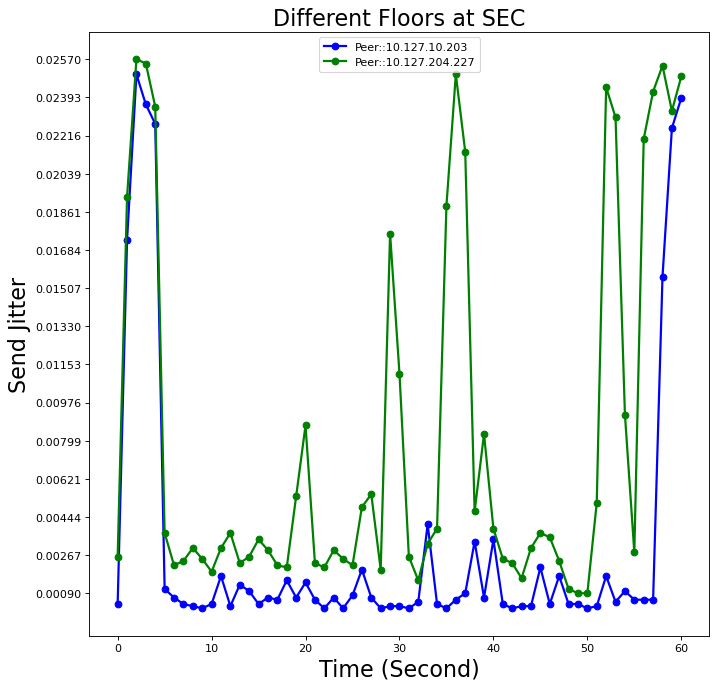
\includegraphics[scale=0.38]{Images/experiment/senarios/df_diff_floor.png}
			%			\vspace{2mm}
		\end{minipage}
		\caption{Jitter values for the time spend by callers}
		\label{fig:scene-out-3}
	\end{figure}


	In the senario 4 (\hyperref[fig:scene-4]{Figure \ref{fig:scene-4}}), peer `A' (IP::10.127.204.227) and peer `B' (IP::10.127.10.203) are calling from different loaction.
	\begin{figure}[thb]
		\begin{minipage}{\textwidth}
			%			\vspace{2mm}
			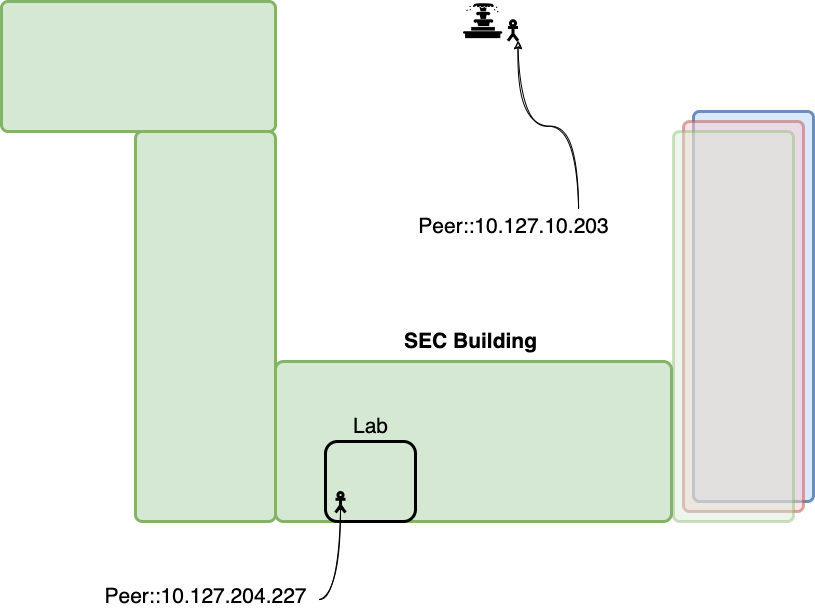
\includegraphics[scale=0.29]{Images/experiment/senarios/near_fountain.drawio.png}
			%			\vspace{2mm}
		\end{minipage}
		\caption{Senario 4: Two peers are at different locations but close access points}
		\label{fig:scene-4}
	\end{figure}

	\begin{figure}[!t]
		\begin{minipage}{\textwidth}
			%			\vspace{2mm}
			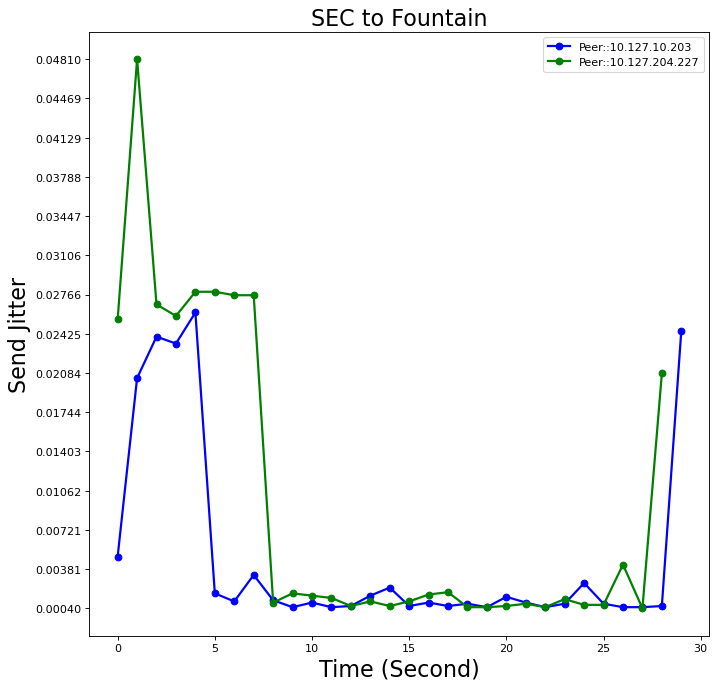
\includegraphics[scale=0.38]{Images/experiment/senarios/df_fountain.png}
			%			\vspace{2mm}
		\end{minipage}
		\caption{Jitter values for the time spend by callers}
		\label{fig:scene-out-4}
	\end{figure}


	In the senario 5 (\hyperref[fig:scene-5]{Figure \ref{fig:scene-5}}), peer `A' (IP::10.127.204.227) and peer `B' (IP::10.127.10.203) are calling from different loaction.
	\begin{figure}[!bh]
		\begin{minipage}{\textwidth}
			%			\vspace{2mm}
			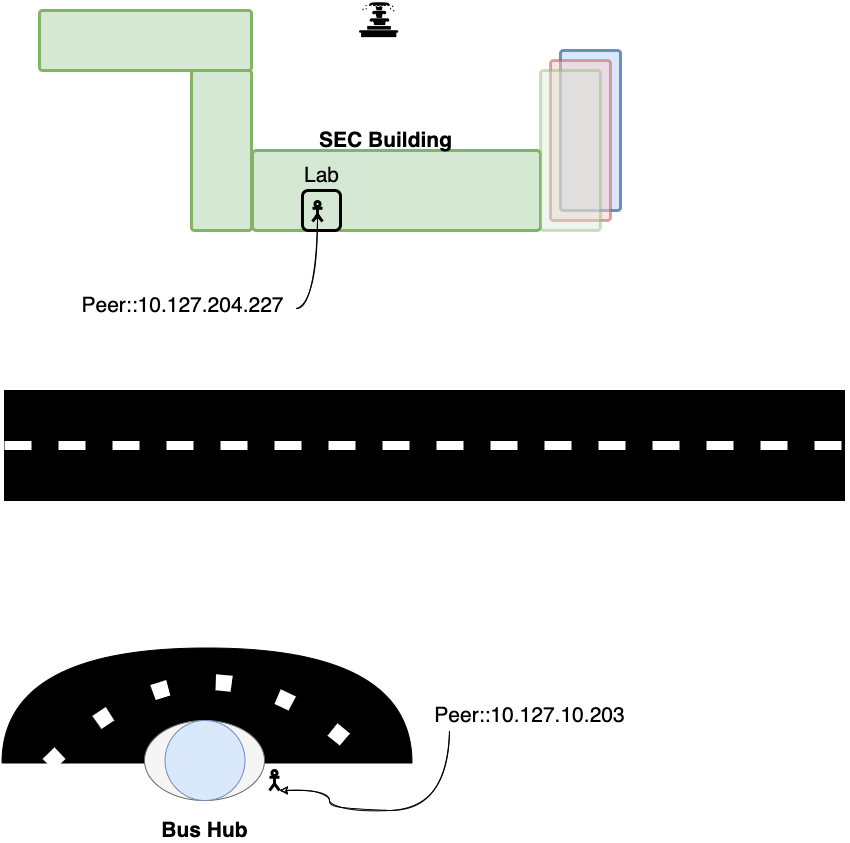
\includegraphics[scale=0.29]{Images/experiment/senarios/bus_hub.drawio.png}
			%			\vspace{2mm}
		\end{minipage}
		\caption{Senario 5: Two peers are at different locations and different building access point}
		\label{fig:scene-5}
	\end{figure}

	\begin{figure}[!t]
		\begin{minipage}{\textwidth}
			%			\vspace{2mm}
			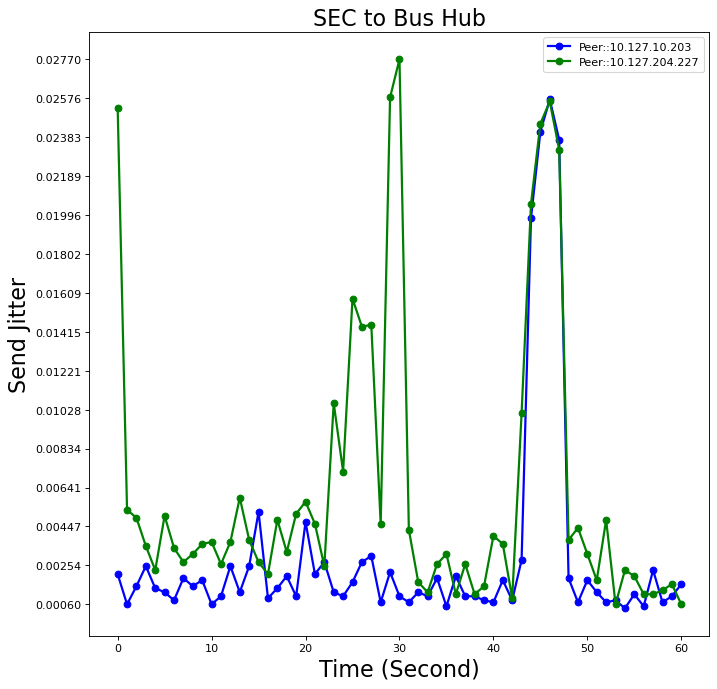
\includegraphics[scale=0.38]{Images/experiment/senarios/df_bus_hub.png}
			%			\vspace{2mm}
		\end{minipage}
		\caption{Jitter values for the time spend by callers}
		\label{fig:scene-out-5}
	\end{figure}